\providecommand{\currentcourse}{Cours 2}
\documentclass[french,t,handout,xcolor=svgnames]{beamer}
\input beamer-header

\begin{document}
\course{1}
\begin{frame}
  \frametitle{$x^{k}x^{l} = x^{k+l}$ ($x\in\RR$ et $k,l \in \NN$)}
  
\end{frame}
\begin{frame}
  \frametitle{S'il pleut ou s'il grèle, je prends mon parapluie.}
  
\end{frame}
% \begin{frame}
%   \frametitle{Chaussettes}
  
% \end{frame}
% \begin{frame}
%   % \begin{question}
%   %   Existe-t-il un nombre qui, multiplé par \(0\), vaut \(1\) ?
%   % \end{question}
  
% \end{frame}
\begin{frame}{Table de vérité $(\neg Q) \ldonc (\neg P)$.}
  
\end{frame}
\course{2}
\begin{frame}{Table de vérité}{$P\land Q$}
  
\end{frame}
\begin{frame}{Table de vérité}{$P\lor Q$}
  
\end{frame}
\begin{frame}{Table de vérité}{$P\ldonc Q$}
  
\end{frame}
\begin{frame}{Dénombrement}{Puissances}
  
\end{frame}
\begin{frame}{Dénombrement}{Arrangements}
  
\end{frame}
\begin{frame}{Dénombrement}{Combinaisons}
  
\end{frame}
\course{3}
\begin{frame}{Inégalités et valeur absolue}{Résoudre : $\abs {x-1} < 1$}

\end{frame}
\begin{frame}{Inégalités et valeur absolue}{Résoudre : $\abs {x-1} < x$}

\end{frame}
\begin{frame}{Inégalités et valeur absolue}{Résoudre : $\abs {x-1} < \abs{x+1}$}

\end{frame}
\begin{frame}{Géométrie}{Système de coordonnées cartésiennes}

\end{frame}
\begin{frame}{Géométrie}{Vecteur libre vs vecteur lié}

\end{frame}
% \course{4}
%% n'a pas été utilisé car pb de compilation puis avec la tablette.
% \begin{frame}{Droites}
  
% \end{frame}
% \begin{frame}
%   \begin{center}
%     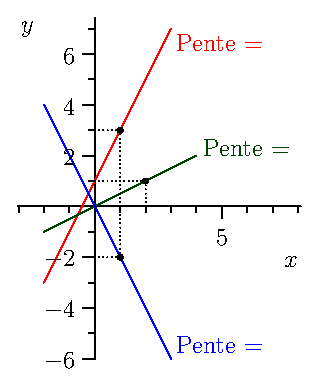
\includegraphics{pentes-sans-pente}
%   \end{center}
% \end{frame}
% \begin{frame}{Angles}
  
% \end{frame}
\course{5}
\begin{frame}{Trigonométrie dans un triangle}
  
\end{frame}
\begin{frame}{}
  
\end{frame}
\course{6} % Fin module A
\begin{frame}{Modification des groupes d'exercices}
  Les groupes en CHIM, INFO et IRBI sont modifiés pour Math F 112 ! Les détails sont sur l'UV.

  Attention en INFO1 le changement prend effet aujourd'hui !
  \begin{description}
  \item[{INFO1}] \alert{dès ce vendredi 2 octobre} (semaine 3)
    \begin{itemize}
    \item Groupe "A et D à H" -- Forum A (Lundi), et OF 2072 (Vendredi)
    \item Groupe "B et I à O" -- NO 506 (Lundi), et NO707 (Vendredi)
    \item Groupe "C et P à Z" -- A2.122 (Lundi), et A2.122 (Vendredi)
    \end{itemize}
  \end{description}

  Comparez régulièrement ces informations avec GeHoL.

  Normalement votre local doit apparaître dans votre horaire (en fait tous les locaux doivent y apparaître !).
\end{frame}


\begin{frame}{Périodicité}
  Soit $f : A \subset \RR \to B$ une fonction.%  Soit un fonction f : A \subset R -> R. On dit qu'elle est périodique si il existe p \in R tel que f(x + p) = f(x) pour tout x \in A. En d'autres termes, le graphe est invariant par translation horizontale d'une longueur p. Un tel nombre p est une *période* de f.

  % Par exemple : sin(x) = sin(x + 2pi) pour tout x.
  % cos(x) = cos(x + 2pi)
  % tan(x) = sin(x)/cos(x) = sin(x+2pi)/cos(x+2pi) = tan(x+2pi), donc 2pi est une période de tan. MAIS
  % tan(x+pi) = sin(x+pi)/cos(x+pi) = -sin(x)/-cos(x) = tan(x), donc pi est *aussi* une période de tan.

  % déf : *la* période d'une fonction périodique f est la plus petite période p > 0.
  % si f(x) = 3 (fonction constante), alors f(x) = 3 = f(x+p) pour tout p. Quelle est la plus petite période p > 0 ? Il n'y en a pas !
  % mind. blown.
  % si f = fonction caractéristique de Q. même question. mind. blown. again.
\end{frame}
\begin{frame}{PPCM}
    \begin{definition}
      Si \(a, b > 0\), leur \og plus petit multiple commun\fg{}, noté \(\ppcm(a,b)\) s'il existe, est le plus petit réel positif qui soit à la fois multiple entier de \(a\) et de \(b\).{} Lorsque le \(\ppcm\) n'existe pas, on dit que \(a\) et \(b\) sont incommensurables.
  \end{definition}
  \begin{example}
    \begin{itemize}
    \item \(\ppcm(3,6) = \)
    \item \(\ppcm(4,6) = \)
    \item \(\ppcm(2\pi,3\pi) = \)
    \item \(\ppcm(4\pi,3\pi) = \)
    \item \(\ppcm(2\pi/3,\pi) = \)
  \end{itemize}
  \end{example}
\end{frame}
\begin{frame}
  \frametitle{Résultats sur la périodicité}
  Si \(p\) est une période de \(f\), \(q\) une période de \(g\), \(h\) une fonction quelconque, et \(c\) une constante réelle :
  \begin{enumerate}[<+->]
  \item Pour la composée \(h\circ f\) : \(p\) est une période de \(h\circ f\) ;
  \item \(f\circ h\) n'est pas a priori périodique (mais peut l'être quand même) ;
  \item \(x \mapsto f(x+c)\) est périodique de période \(p\)% (un des rares cas où l'on est sûr de \emph{la} période !) ;
  \item \(x \mapsto f(cx)\) est périodique de période \(\frac pc\)% (un autre rare cas) ;
  \item \(f+g\), \(fg\), \(f/g\) admettent \(\ppcm(p,q)\) comme période (pas forcément la plus petite).
  \end{enumerate}
  \begin{example}
    Une période de \(\sin(3x) + \cos(2x)\) est
  \end{example}
\end{frame}

\begin{frame}{Période de $\sin(x^{2})$}
 Cette fonction n'admet pas de période.
\end{frame}
\begin{frame}{Injection}
  Soit $f : A \subset \RR \to B$ une fonction.
  

\end{frame}
\begin{frame}{Ensemble image}
  Soit $f : A \subset \RR \to B$ une fonction. L'\emph{ensemble image} de $f$ est

  \vspace{2cm}

  \begin{itemize}
  \item $\RR \to \RR : x \mapsto x^{2}$. Alors $\Im f = $
  \item $\RR \to \RR : x \mapsto \sin (x)$. Alors $\Im f = $
  \item $\interoo{-\pi/2,\pi/2} \to \RR : x \mapsto \tan (x)$. Alors $\Im f = $
  \end{itemize}
\end{frame}
\begin{frame}{Surjection}
  Soit $f : A \subset \RR \to B$ une fonction.  
\end{frame}
\begin{frame}{Inversibilité}
  Soit $f : A \subset \RR \to B$ une fonction.

\end{frame}
\begin{frame}{Tangente, cosinus, sinus et leur inverse}
  
\end{frame}
\begin{frame}{Exponentielles vs logarithmes}

\end{frame}

\section{Géométrie dans l'espace}
\begin{frame}{Droite et vecteur normal}
  Dans le plan, une droite passant par $(p_1,p_2)$ dans la direction $(v_1,v_2)$ a pour équation $v_2 x - v_1 y + p_2v_1-p_1v_2 = 0$.

  En général, regardons la droite d'équation $ax+by + c = 0$.
\end{frame}
\begin{frame}{Plans dans l'espace}
  L'équation d'un plan passant par $\point p$ dans l'espace est :
  \begin{equation*}
    \scalprod{(a,b,c)}{(x,y,z) - (p_1,p_2,p_3)} = 0
  \end{equation*}
  
  Équation générale : $ax+by+cz + d = 0$.
\end{frame}
\begin{frame}{Orientabilité}
  
\end{frame}
\begin{frame}
  \frametitle{Produit vectoriel}
  
\end{frame}
\begin{frame}{Propriété du produit vectoriel}
\begin{proposition}Le produit vectoriel vérifie les identités suivantes~:
    \begin{itemize}
    \item \(\vec a \vecprod \vec b \perp \vec a\) et \(\vec a \vecprod \vec b \perp \vec b\);
    \item \(\norme{\vec a \vecprod \vec b}^{2} + \abs{\scalprod{\vec a }{\vec b}}^{2} = \norme {\vec a}^{2} \norme{\vec b}^{2}\);
    \item \(\norme{\vec a \vecprod \vec b} = \norme {\vec a} \norme{\vec b} \sin \theta \) ;
    \item \(\vec a \vecprod \vec b = -\vec b \vecprod \vec a\) (anti-symétrique) ;
    \item \((\alpha \vec {a} + \alpha' \vec{a'}) \vecprod \vec b = \alpha {\vec a \vecprod \vec b} + \alpha' {\vec {a'} \vecprod \vec b}\)
    \end{itemize}
    pour tout \(\alpha, \alpha' \in \RR\) et \(\vec a, \vec {a'}, \vec b \in \RR^{3}\), et où \(\theta\) est l'angle formé par les vecteurs \(\vec a\) et \(\vec b\).
  \end{proposition}
  
  De plus les vecteurs $\vec a, \vec b, \vec a \vecprod \vec b$ sont orientés comme le trièdre $(1,0,0), (0,1,0), (0,0,1)$.
\end{frame}

\begin{frame}{Distance point-droite dans le plan}

\end{frame}
\begin{frame}{Distance point-plan dans l'espace}
  Soit un plan d'équation
  \begin{equation*}
    a x + b y + c z + d = 0.
  \end{equation*}
  La distance entre ce plan et le point \(\point{p}\) est
  \begin{equation*}
    \frac{\abs{a p_{1} + b p_{2} + c p_{3} + d}}{\sqrt{a^{2} + b^{2} + c^{2}}}
  \end{equation*}
\end{frame}
\begin{frame}{Coordonnées polaires}
  
\end{frame}
\course{7} % Début module T
\begin{frame}{Fonctions réelles}{Introduction aux limites}
  
\end{frame}

\begin{frame}{Limites}{Adhérence}
  
\end{frame}
\begin{frame}{Limites}{Définition de limite finie en $x = a$}
  
\end{frame}
\begin{frame}{Limites}{Exemples de limite finie}
  
\end{frame}
\begin{frame}{Limites}{Définition de limite infinie en $x = a$}
  
\end{frame}
\begin{frame}{Limites}{Exemples de limite infinie}
  
\end{frame}
\begin{frame}{Limites}{Limite à gauche, limite à droite}
  
\end{frame}
\begin{frame}{Limites}{Fonction continue}

\end{frame}
\begin{frame}{Limites}{Opérations / règles de calcul}
  
\end{frame}

\begin{frame}{Limites}{Exemples de calcul}
  
\end{frame}
\begin{frame}{Parenthèse sur la division euclidienne}{Racines et polynômes}%% déjà connu des étudiants!
  
  
\end{frame}
\begin{frame}{Parenthèse sur la division euclidienne}{Algorithme de division}
  
\end{frame}
\begin{frame}{Parenthèse sur la division euclidienne}{Exemple}
  
\end{frame}
\course{8}
\begin{frame}{Limites}{Règles étendues à l'infini}
  %% Soit f une fct, et a \in \adh \dom f
  %% si f(x) \to \infty, alors 1/f(x) \to 0;
  %% De manière concise on écrit:   1/\infty = 0. Mais c'est un nouveau résultat qui ne découle *pas* des résultats précédents.
  %% si f(x) \to 0^+ alors 1/f(x) \to +\infty
  %% rem: on dit f(x) \to 0^ si f(x) \to 0 et si f(x) > 0 pour tout x près de a (c'est-à-dire qu'il existe delta t.q. f(x) > 0 pour x \in \interoo{a-\delta, a+\delta} \cap \dom f).
  %% par exemple x^2 \to 0^+ mais on n'a pas sin(x) \to 0^+. Par contre lim_(x\to 0\\ x > 0) sin(x) = 0^+ (i.e. limite à droite).
  %% si f(x) \to 0^- alors 1/f(x) \to -\infty
  %% Encore, on écrira parfois: 1/0^+ = +\infty et 1/0^- = -\infty
  %% Similairement nous pouvons énoncer des résultats qui s'écrivent de manière concise:
  %%
% \begin{align*}
%   \frac{L}{0^+}&=
%   \begin{cases}
%     + \infty &\textrm{si } L > 0\\
%     - \infty &\textrm{si } L < 0
%   \end{cases}&
%   \frac{L}{0^-}&=
%   \begin{cases}
%     - \infty &\textrm{si } L > 0\\
%     + \infty &\textrm{si } L < 0
%   \end{cases}\\
%   \frac{\pm \infty}{0^+}&=\pm \infty&
%   \frac{\pm \infty}{0^-}&=\mp \infty \text{ (changement de signe !)}
% \end{align*}

  %% les combinaisons suivantes sont des "formes indéterminées" : ∞ - ∞, 0∞, ∞/∞, 0/0, 1^∞, ∞⁰, 0⁰
\end{frame}
\begin{frame}{Limites en l'infini}
  %  Jusqu'à présent on a regardé $x \to a$. On peut aussi regarder $x \to \infty$.
  % Exemple lim f(x) = L si x \to infty est défini par:
  % ...
\end{frame}
\begin{frame}{D'autres exemples de limites}
  % (x^2 + 1)/(x^2 -1)
  % \exp{1/x} tend vers 0 pour x \to 0^- et vers +\infty pour x \to 0^+
  % arctan(x) tend vers -pi/2 si x \to -\infty.
\end{frame}
\begin{frame}{Notation de Landau et ordre de grandeur}
  % On peut vouloir comparer l'évolution de deux fonctions f et g lorsque x s'approche de l'infini.
  
  % définition: on dit que f est un O(g(x)) si il existe une constante C et un réel r tel que pour x > r, on a |f(x)| ≤ C |g(x)|.
  % on dit aussi que f est d'un ordre de grandeur (asymptotique) inférieur à g.
  % exemple: x^n est un O(x^m) si n \leq m.
  % x^n est un O(e^x) pour toute valeur de n.
  % N.B.: bien que 2x > x pour tout x > 0, on a bien: 2x est un O(x) ! En fait on a aussi: x est un O(2x).
  % quand f(x) est O(g(x)) et g(x) est O(f(x)), on dit que f et g sont asymptotiquement du même ordre.

  % Comment prouver ces affirmations ? On a un résultat :
  % si la limite |f(x)/g(x)| est réelle, alors f(x) est un O(g(x)).
  % si la limite |f(x)/g(x)| est infinie, alors f(x) n'est pas un O(g(x)) (par contre g(x) est un O(f(x))).
  % Il est aussi possible que cette limite n'existe pas !

  % Preuve : si la limite est réelle, disons L, alors il existe r t.q. si x > r, on a : ||f(x)/g(x)| - L|
\end{frame}
\begin{frame}{Notion de petit o}
  %  Une notion similaire est celle de petit o :
  % on dit que f(x) est o(g(x)) (pour x \to a, ou x \to \infty) si f(x)/g(x) tend vers 0 (pour x \to a, ou x \to \infty).
  % rem: si f(x) est o(g(x)) alors f(x) est O(g(x)) d'après le résultat précédent.
\end{frame}
\begin{frame}{Théorème du Sandwich}
  % si f(x) \leq g(x) \leq h(x) ; et si f(x) et h(x) tendent vers une même limite L (ou ±∞) quand x tend vers a (ou ±∞)
  % alors g(x) tend vers L aussi.
  % faisons la preuve dans le cas où a et L sont des réels.
  % hypothèses :
  % ∀ε > 0 ∃ δ₁ > 0 : ∀x (|x-a| < δ₁ → |f(x)-L| < ε)
  % ∀ε > 0 ∃ δ₂ > 0 : ∀x (|x-a| < δ₂ → |h(x)-L| < ε)
  % On veut :
  % ∀ε > 0 ∃ δ > 0 : ∀x (|x-a| < δ → |g(x)-L| < ε)
  % Soit ε > 0. On prend δ₁ et δ₂ tels que ci-dessus.
  % On définit alors δ = min(δ₁,δ₂). Alors pour |x-a| < δ on a:
  % |f(x) - L| < ε et |f(x) - L| < ε
  % c'est-à-dire: -ε < f(x) - L < ε et -ε < h(x) - L < ε
  % Donc on a :
  % -ε < f(x) - L ≤ g(x) - L ≤ h(x) - L < ε
  % dès lors |g(x) - L| < ε comme attendu !
\end{frame}
\begin{frame}{Théorème de la valeur intermédiaire}
  %  On aimerait que si $f(a) < 0$ et $f(b) > 0$, alors quelque part entre a et b, il existe c avec $f(c) = 0$. Ce rêve devient réalité si f est continue sur l'intervalle $[a,b]$.
  % Si f : [a,b] \to \RR est continue, alors pour tout $\gamma$ entre $f(a)$ et $f(b)$ il existe $c \in \interoo{a,b}$
  % La preuve, un peu technique, est omise.
  
  % exemple : tout polynôme de degré impair admet au moins une racine réelle.
  % en effet, considérons P(x)= a_0 + a_1 x + a_2 x^2 + ... + a_n x^n avec a_n \neq 0 et n impair.
  % Les racines de $P$ sont les $x$ tels que $P(x) = 0$. En divisant par a_n, on peut supposer $a_n = 1$.
  % Notons alors que $P(x) = x^{n} (a_0/x^{n} + a_1 x/x^{n} + ... + x^{n}/x^{n})$ et donc
  % lim x \to \pm\infty P(x) = \pm\infty$
\end{frame}
\begin{frame}{Théorème des bornes atteintes}
  % Si f : [a,b] \to \RR est continue, alors il existe $m, M \in [a,b]$ avec $f(m) \leq f(x) \leq f(M)$. Entre d'autres termes $f(m)$ est le minimum de $f$ sur l'intervalle, et $f(M)$ est son maximum.
  % La preuve, très technique, est omise.

  % n.b.: si on considère f : \interoo{0,1} \to \RR : x \mapsto x, elle n'admet pas de minimum ou de maximum car on a exclu 0 et 1 du domaine ! D'où l'importance que les bords du domaine soient dedans.
\end{frame}
\begin{frame}{Théorème de la fonction réciproque}
  % si f: I \to J une bijection *continue* où $I$ est un intervalle (et alors, forcément, $J$ aussi).
  % alors f^(-1) : J \to I est encore continue.
  % La preuve est omise.
\end{frame}

%%% À faire un jour ?
% Aire d'un triangle via produit vectoriel.
% Preuve de distance point-droite ?
% Preuve de distance point-plan ?
% distance droite-plan ?
% angle droite-droite
% angle droite-plan

%% Diagrammes de Venn.
%% Exemple: A \cap (B \cup C) = (A\cap B) \cup (A\cap C)


\end{document}

%%% Local Variables:
%%% TeX-master: t
%%% eval: (yf/narrow-to-course-mode)
%%% page-delimiter: "^\\\\course.*"
%%% sentence-end-base: "[.?!][]\"'”)}]*\\(?:\\\\\\)?\\(?:{}\\)?"
%%% TeX-engine: luatex
%%% End:
